\documentclass[]{exam}
\usepackage{epic,array,ecltree,url,calrsfs}
\usepackage[nointegrals]{wasysym}

%These tell TeX which packages to use.
\usepackage{array,epsfig}
\usepackage{amsmath}
\usepackage{amsfonts}
\usepackage{amssymb}
\usepackage{amsxtra}
\usepackage{amsthm}
\usepackage{mlextra} % must come after ams packages
\usepackage{mathrsfs}
\usepackage[dvipsnames]{xcolor}
\usepackage{array}
\usepackage{graphicx}
\graphicspath{ {../art/} }
\usepackage{bm}
\usepackage{tikz}
\usepackage{multicol}
\usepackage{enumitem}

\newcommand{\twonode}{%
  \begingroup\normalfont
  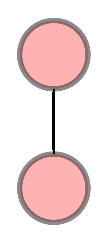
\includegraphics[height=\fontcharht\font`\b]{2nodetree.eps}%
  \endgroup
}


\title{Lab 5: Validity, Satisfiability, Normal Forms}
\author{Foundations of Computer Science}
\date{\today}
%\pagestyle{empty} 
%\footer{}{\thepage}{}
\unframedsolutions
\SolutionEmphasis{\itshape\small}
\SolutionEmphasis{\color{NavyBlue}}


\begin{document}

\maketitle

\setlength{\columnseprule}{1pt}
\begin{questions}

\question Answer the questions below for the formula $A$, where $A \equiv (p \imp q)
  \eqv (\ngg p \imp \ngg q)$.
\begin{parts}
\part What is $\mathcal{P}_A$? 
\begin{solution}
$\{p,q \}$
\end{solution}

\part Define $\mathcal{I}_A: \mathcal{P}_A \to \{T,F\}$ as $\mathcal{I}_A(p) =
T$, $\mathcal{I}_A(q) = F$.  Is $\mathcal{I}_A$ a model for $A$?
\begin{solution}
No.
\end{solution}

\part Give an interpretation that satisfies $A$ or prove $A$ is not
satisfiable.
\begin{solution}
$\mathcal{I}_A(p) = T$, $\mathcal{I}_A(q) = T$ or $\mathcal{I}_A(p) = F$, $\mathcal{I}_A(q) = F$ \\
\end{solution}
\end{parts}


\question Answer the questions below for the formula $A$, where $A \equiv ((p \imp q) \imp q) \imp q$.
\begin{parts}
\part What is $\mathcal{P}_A$? 
\begin{solution}
$\{p,q \}$
\end{solution}

\part Define $\mathcal{I}_A: \mathcal{P}_A \to \{T,F\}$ as $\mathcal{I}_A(p) =
T$, $\mathcal{I}_A(q) = T$.  Is $\mathcal{I}_A$ a model for $A$?
\begin{solution}
Yes.
\end{solution}

\part Is $A$ satisfiable?
\begin{solution}
Yes.
\end{solution}

\part Prove $\models A$ or give an interpretation that falsifies $A$.
\begin{solution}
$\mathcal{I}_A(p) = T$, $\mathcal{I}_A(q) = F$ 
\end{solution}
 
\end{parts}

\question Answer the questions below for the formula $A$, where $A \equiv (p \eqv q) \eqv (p \eqv (q \eqv p))$.
\begin{parts}
\part Give an interpretation that satisfies $A$.
\begin{solution}
$\mathcal{I}_A(p) = T$, $\mathcal{I}_A(q) = T$ or $\mathcal{I}_A(p) = T$, $\mathcal{I}_A(q) = F$
\end{solution}
\part Prove $A$ is valid or give an interpretation that falsifies $A$.
\begin{solution}
$\mathcal{I}_A(p) = F$, $\mathcal{I}_A(q) = F$ or $\mathcal{I}_A(p) = F$, $\mathcal{I}_A(q) = T$
\end{solution}
\end{parts}

\question Answer the questions below for the formula $A$, where $A \equiv ((p \land q) \imp
    r) \imp ((p \imp r) \lor (q \imp r))$ 
\begin{parts}
\part\label{p:nnf} Change $A$ to Negation Normal Form. 
\begin{solution}
\begin{align*}
&((p \land q) \imp r) \imp ((p \imp r) \lor (q \imp r)) & \text{original} \\
&\equiv \ngg (\ngg (p \land q) \lor r) \lor ((\ngg p \lor r) \lor (\ngg q \lor r))& \text{eliminate ``}\imp \text{'' symbols} \\
&\equiv ( (p \land q) \land \ngg r) \lor ((\ngg p \lor r) \lor (\ngg q \lor r))& \text{distribute negation} \\
&\equiv ((p \land q) \land \ngg r) \lor (\ngg p \lor r \lor \ngg q)& \text{simplify} 
\end{align*}

\end{solution}
\part\label{p:cnf} Change $A$ to Conjunctive Normal Form.
\begin{solution}
\begin{align*}
&((p \land q) \imp r) \imp ((p \imp r) \lor (q \imp r)) & \text{original} \\
&\equiv ((p \land q) \land \ngg r) \lor (\ngg p \lor r \lor \ngg q)& \text{NNF (see above)} \\
&\equiv ( (p \land q)\lor (\ngg p \lor r \lor \ngg q )) \land (\ngg r \lor (\ngg p \lor r \lor \ngg q )) & \text{distribute over } \land \\
&\equiv ( (p \lor (\ngg p \lor r \lor \ngg q )) \land (q \lor (\ngg p \lor r \lor \ngg q ) )) \land (\ngg r \lor (\ngg p \lor r \lor \ngg q )) & \text{distribute over } \land \\
&\equiv ( (p \lor \ngg p \lor r \lor \ngg q ) \land (q \lor \ngg p \lor r \lor \ngg q )) \land (\ngg r \lor \ngg p \lor r \lor \ngg q ) & \text{remove unneeded parentheses } \\
&\equiv (p \lor \ngg p \lor r \lor \ngg q ) \land (q \lor \ngg p \lor r \lor \ngg q ) \land (\ngg r \lor \ngg p \lor r \lor \ngg q ) & \text{CNF } \\
\end{align*}
\end{solution}
\part Prove $\models A$.
\begin{solution}
~\\
    By parts (\ref{p:nnf}) and (\ref{p:cnf}) above we have \[
A \equiv (p \lor \ngg p \lor r \lor \ngg q ) \land (q \lor \ngg p \lor r \lor \ngg q  ) \land (\ngg r \lor \ngg p \lor r \lor \ngg q )
  \]
  Simplifying each of the three conjunctions, we find:
\begin{align*}
  (p \lor \ngg p \lor r \lor \ngg q ) &\equiv ((p \lor \ngg p) \lor r \lor \ngg q) \equiv (\top \lor r \lor \ngg q ) \equiv \top & \text{1st conjunction} \equiv \top\\
  (q \lor \ngg p \lor r \lor \ngg q ) & \equiv ((q \lor \ngg q) \lor \ngg p \lor r) \equiv (\top \lor \ngg p \lor r ) \equiv \top & \text{2nd conjunction} \equiv \top \\
  (\ngg r \lor \ngg p \lor r \lor \ngg q ) &\equiv ((\ngg r \lor r) \lor \ngg p \lor \ngg q ) \equiv (\top \lor \ngg p \lor \ngg q ) \equiv \top & \text{3rd conjunction} \equiv \top\\
\end{align*}
Therefore, $A \equiv \top \land \top \land \top \equiv \top$ 
\end{solution}

\part Show that $\ngg A$ is unsatisfiable.
\begin{solution}
By theorem (2.39) in Ben Ari, $\ngg A$ is unsatisfiable if and only if $A$ is
valid. We have proved that $A$ is valid in the previous problem, so $\ngg A$ is unsatisfiable.
\end{solution}
\end{parts}

\question Answer the questions below for the formula $A$, where 
          $A \equiv (p \imp q) \lor (q \imp r)$ 

\begin{parts}

\part Change $A$ to Negation Normal Form. 
\begin{solution}
\begin{align*}
A &\equiv (p \imp q) \lor (q \imp r) &\text{original} \\
 &\equiv (\ngg p \lor q) \lor (\ngg q \lor r) &\text{eliminate ``}\imp \text{'' symbols} 
\end{align*}
\end{solution}

\part Change $A$ to Conjunctive Normal Form.
\begin{solution}
\begin{align*}
A &\equiv (p \imp q) \lor (q \imp r) &\text{original} \\
 &\equiv (\ngg p \lor q) \lor (\ngg q \lor r) &\text{NNF (see above)} \\ 
 & \equiv \ngg p \lor q \lor \ngg q \lor r &\text{eliminate unneeded parentheses} 
\end{align*}
\end{solution}

\part Prove $\models A$.
\begin{solution}
\begin{align*}
A &\equiv (\ngg p \lor q \lor \ngg q \lor r) &\text{CNF (see above)}\\
   &\equiv (\ngg p \lor (q \lor \ngg q) \lor r)&\text{associative property} \\
   &\equiv (\ngg p \lor \top \lor r)& A \lor \ngg A \equiv \top \\
   &\equiv \top & \top \lor A \equiv \top 
\end{align*}
\end{solution}

\part Show that $\ngg A$ is unsatisfiable.
\begin{solution}
Again, by theorem (2.39) in Ben Ari, $\ngg A$ is unsatisfiable if and only if $A$ is
valid. 
\end{solution}
\end{parts}

\question\label{q:bigCNF} Change $A$ to Conjunctive Normal Form. 
\begin{parts}

\part\label{q:4lit} $A \equiv (p_1 \land q_1) \lor (p_2 \land q_2)$.
\begin{solution}
\begin{align*}
A &\equiv (p_1 \land q_1) \lor (p_2 \land q_2).\\
  &\equiv (p_1 \lor (p_2 \land q_2)) \land (q_1 \lor (p_2 \land q_2)).\\
  &\equiv (p_1 \lor p_2) \land (p_1 \lor q_2) \land (q_1 \lor p_2) \land (q_1 \lor q_2).\\
\end{align*}
\end{solution}

\part\label{q:6lit} $A \equiv (p_1 \land q_1) \lor (p_2 \land q_2) \lor (p_3 \land q_3)$.
\begin{solution}
\begin{align*}
 A &\equiv& &(p_1 \land q_1) \lor (p_2 \land q_2) \lor (p_3 \land q_3)\\
 &\equiv& &((p_1 \lor p_2) \land (p_1 \lor q_2) \land (q_1 \lor p_2) \land (q_1 \lor q_2)) 
                                                                    \lor (p_3 \land q_3) 
                                                  &\text{ by part (\ref{q:4lit}) above}\\
 %%%%%%%%%%%%%%
 &\equiv& &(((p_1 \lor p_2) \land (p_1 \lor q_2) \land (q_1 \lor p_2)) \lor (p_3 \land q_3)) 
                                               \land ((q_1 \lor q_2) \lor (p_3 \land q_3))
                                                  &\text{distribute }(p_3 \land q_3)\\
 %%%%%%%%%%%%%%
 &\equiv& &(((p_1 \lor p_2) \land (p_1 \lor q_2) \land (q_1 \lor p_2)) \lor (p_3 \land q_3)) 
                         \land (((q_1 \lor q_2) \lor p_3) \land ((q_1 \lor q_2) \lor q_3)) 
                                                       &\text{distribute }(q_1 \lor q_2)\\
 %%%%%%%%%%%%%%
 &\equiv& &(((p_1 \lor p_2) \land (p_1 \lor q_2) \land (q_1 \lor p_2)) \lor (p_3 \land q_3)) 
                               \land (q_1 \lor q_2 \lor p_3) \land (q_1 \lor q_2 \lor q_3) 
                                                                        &\text{simplify}\\
 %%%%%%%%%%%%%%
 &\equiv& &((((p_1 \lor p_2) \land (p_1 \lor q_2)) \land (q_1 \lor p_2)) \lor (p_3 \land q_3)) 
                                                                        &\text{associate}\\
 & & & \land (q_1 \lor q_2 \lor p_3) \land (q_1 \lor q_2 \lor q_3) \\
 %%%%%%%%%%%%%%
  &\equiv& &(((((p_1 \lor p_2) \land (p_1 \lor q_2)) \lor (p_3 \land q_3)))
                               \land ((q_1 \lor p_2) \lor (p_3 \land q_3))) 
                                                        &\text{distribute }(p_3 \land q_3)\\
 & & & \land (q_1 \lor q_2 \lor p_3) \land (q_1 \lor q_2 \lor q_3) \\
 %%%%%%%%%%%%%%
  &\equiv& &(((((p_1 \lor p_2) \land (p_1 \lor q_2)) \lor (p_3 \land q_3)))
                               \land (((q_1 \lor p_2) \lor p_3) \land ((q_1 \lor p_2) \lor q_3))) 
                                                        &\text{distribute }(q_1 \lor p_2)\\
 & & & \land (q_1 \lor q_2 \lor p_3) \land (q_1 \lor q_2 \lor q_3) \\
 %%%%%%%%%%%%%%
  &\equiv& &(((p_1 \lor p_2) \land (p_1 \lor q_2)) \lor (p_3 \land q_3))
                                                        &\text{simplify } \\
 & & & \land (q_1 \lor p_2 \lor p_3) \land (q_1 \lor p_2 \lor q_3) 
       \land (q_1 \lor q_2 \lor p_3) \land (q_1 \lor q_2 \lor q_3) \\
 %%%%%%%%%%%%%%
  &\equiv& &(((p_1 \lor p_2)\lor (p_3 \land q_3)) \land ((p_1 \lor q_2)\lor (p_3 \land q_3)))
                                                        &\text{distribute }(p_3 \land q_3)\\
 & & & \land (q_1 \lor p_2 \lor p_3) \land (q_1 \lor p_2 \lor q_3) 
       \land (q_1 \lor q_2 \lor p_3) \land (q_1 \lor q_2 \lor q_3) \\
 %%%%%%%%%%%%%%
  &\equiv& &(((p_1 \lor p_2)\lor (p_3 \land q_3)) \land 
            (((p_1 \lor q_2) \lor p_3) \land
             ((p_1 \lor q_2) \lor q_3)))
                                                        &\text{distribute }(p_1 \lor q_2)\\
 & & & \land (q_1 \lor p_2 \lor p_3) \land (q_1 \lor p_2 \lor q_3) 
       \land (q_1 \lor q_2 \lor p_3) \land (q_1 \lor q_2 \lor q_3) \\
 %%%%%%%%%%%%%%
 &\equiv& &(((p_1 \lor p_2)\lor (p_3 \land q_3)) 
       \land (p_1 \lor q_2 \lor p_3) \land (p_1 \lor q_2 \lor q_3)
                                                        &\text{simplify } \\
 & & & \land (q_1 \lor p_2 \lor p_3) \land (q_1 \lor p_2 \lor q_3) 
       \land (q_1 \lor q_2 \lor p_3) \land (q_1 \lor q_2 \lor q_3) \\
 %%%%%%%%%%%%%%
 &\equiv& & (((p_1 \lor p_2)\lor p_3) \land ((p_1 \lor p_2) \lor q_3)) 
      \land (p_1 \lor q_2 \lor p_3) \land (p_1 \lor q_2 \lor q_3)
                                                        &\text{distribute }(p_1 \lor p_2)\\
 & & & \land (q_1 \lor p_2 \lor p_3) \land (q_1 \lor p_2 \lor q_3) 
       \land (q_1 \lor q_2 \lor p_3) \land (q_1 \lor q_2 \lor q_3) \\
 %%%%%%%%%%%%%%
&\equiv& &   (p_1 \lor p_2 \lor p_3) \land (p_1 \lor p_2 \lor q_3) 
       \land (p_1 \lor q_2 \lor p_3) \land (p_1 \lor q_2 \lor q_3)
                                                        &\text{simplify } \\
 & & & \land (q_1 \lor p_2 \lor p_3) \land (q_1 \lor p_2 \lor q_3) 
       \land (q_1 \lor q_2 \lor p_3) \land (q_1 \lor q_2 \lor q_3) \\
 %%%%%%%%%%%%%%
\end{align*}

  
%\equiv (((p_1 \lor p_2) \land (p_1 \lor q_2)) \lor (p_3 \land q_3)) 
% \land (((q_1 \lor p_2) \lor p_3 \land (q_1 \lor p_2) \lor q_3)) 
% \land ((q_1 \lor q_2 \lor p_3) \land (q_1 \lor q_2 \lor q_3).

%\equiv ((p_1 \lor p_2) \land (p_1 \lor q_2) \lor (p_3 \land q_3)) 
% \land ((q_1 \lor p_2 \lor p_3) \land (q_1 \lor p_2 \lor q_3)) 
% \land ((q_1 \lor q_2 \lor p_3) \land (q_1 \lor q_2 \lor q_3).

%\equiv ((p_1 \lor p_2) \lor (p_3 \land q_3)) 
% \land ((p_1 \lor q_2) \lor (p_3 \land q_3)) 
% \land ((q_1 \lor p_2 \lor p_3) \land (q_1 \lor p_2 \lor q_3)) 
% \land ((q_1 \lor q_2 \lor p_3) \land (q_1 \lor q_2 \lor q_3).

%\equiv ((p_1 \lor p_2) \lor p_3 \land q_3) 
% \land ((p_1 \lor q_2) \lor p_3 \land q_3) 
% \land ((q_1 \lor p_2 \lor p_3) \land (q_1 \lor p_2 \lor q_3)) 
% \land ((q_1 \lor q_2 \lor p_3) \land (q_1 \lor q_2 \lor q_3).

%\equiv ((p_1 \lor p_2) \lor p_3 \land (p_1 \lor p_2) \lor q_3) 
% \land ((p_1 \lor q_2) \lor p_3 \land (p_1 \lor q_2) \lor q_3) 
% \land ((q_1 \lor p_2 \lor p_3) \land (q_1 \lor p_2 \lor q_3)) 
% \land ((q_1 \lor q_2 \lor p_3) \land (q_1 \lor q_2 \lor q_3).

%\equiv (p_1 \lor p_2 \lor p_3) \land (p_1 \lor p_2 \lor q_3) 
% \land (p_1 \lor q_2 \lor p_3) \land (p_1 \lor q_2 \lor q_3) 
% \land (q_1 \lor p_2 \lor p_3) \land (q_1 \lor p_2 \lor q_3) 
% \land (q_1 \lor q_2 \lor p_3) \land (q_1 \lor q_2 \lor q_3).

\end{solution}
\end{parts}

\question Let $A$ be a formula of the form $(p_1 \land q_1) \lor (p_2 \land
    q_2)\lor ...\lor (p_n \land q_n)$
\begin{parts}
\part In terms of $n$, how many conjunctions are in $A$?
\begin{solution}
There are $n$ conjunctions (numbered $1$ to $n$).
\end{solution}
\part In terms of $n$, how many literals are in $A$?
\begin{solution}
$2n$
\end{solution}
\part Answer the following questions about the CNF of $A$ based on the pattern 
observed in question \ref{q:bigCNF}:
\begin{subparts}
\subpart How many literals will there be in each disjunction in the CNF of $A$ 
         (in terms of $n$)?
\begin{solution}
$n$. Each disjunction contains one literal from each of the conjunctions in
$A$.
\end{solution}
\subpart How many disjunctions will there be in the CNF of $A$ (in terms of $n$)? 
\begin{solution}
$2^n$. There are two literals in each of the $n$ conjunctions of $A$. Each
disjunction in the CNF of $A$ contains exactly one representative from 
each of the original conjunctions. Subject to these constraints, there is a
disjunction for every possible combination.
\end{solution}
\subpart In total, how many literals will be in the CNF of $A$ (in terms of $n$)?
\begin{solution}
$n(2^n)$
\end{solution}
\end{subparts}
\end{parts}
\question  Using the modified version of the \texttt{Inorder} Function and
the formula \texttt{F1} given below, write the output of \texttt{Inorder(F1,0)}.
List all the calls to \texttt{Inorder} in the order they are made, with the
arguments passed in for each call. (You may want to label subformulas of
\texttt{F1}.)
\begin{verbatim}
Inorder(F,n)
  if F is a leaf
    write its label
    write `['
    write the value of n
    write `]'
    return
  let F1 and F2 be the left and right subtrees of F
  write a left parenthesis `('
  Inorder(F1, n+1)
  write the label of the root of F
  write `['
  write the value of n
  write `]'
  Inorder(F2, n+1)
  write a right parenthesis `)'
\end{verbatim}

\texttt{F1}  \\
\setlength{\GapWidth}{8mm}
\setlength{\GapDepth}{8mm}
\begin{bundle}{$\eqv$}
\chunk{
  \begin{bundle}{$\imp$}
  \chunk{$p$}
  \chunk{$q$}
  \end{bundle}
}
\chunk{
  \begin{bundle}{$\imp$}
  \chunk{
    \begin{bundle}{$\ngg$}
    \chunk{$p$}
    \end{bundle}
  }
  \chunk{
    \begin{bundle}{$\ngg$}
    \chunk{$q$}
    \end{bundle}
  }
  \end{bundle}
}
\end{bundle}\\
\begin{solution}
Let $FL_{\imp}$ and $FR_{\imp}$ refer to the left and right subtrees with $\imp$ as their
primary operator, and $FL_{\ngg}$ and $FR_{\ngg}$ refer to the left and right
subtrees with $\ngg$ as their primary operator. The following table enumerates
the function calls and their arguments on the left. The list on the right shows
the output printed after the function call with the same number on the left, but
before the next function call.
\begin{multicols}{2}
{ \bf Function Calls:}

\begin{enumerate}
\item \texttt{Inorder(F1,0)}
\item \texttt{Inorder($FL_{\imp}$,$1$)}
\item \texttt{Inorder($p$,$2$)}
\item \texttt{Inorder($q$,$2$)}
\item \texttt{Inorder($FR_{\imp}$,$1$)}
\item \texttt{Inorder($FL_{\ngg}$,$2$)}
\item \texttt{Inorder($NULL$,$3$)} (optional) 
\item \texttt{Inorder($p$,$3$)}
\item \texttt{Inorder($FR_{\ngg}$,$2$)}
\item \texttt{Inorder($NULL$,$3$)} (optional) 
\item \texttt{Inorder($q$,$3$)}
\end{enumerate}
\columnbreak
{ \bf Output:}
\begin{enumerate}
\item $($
\item $(($
\item $((p[2] \imp[1]$
\item $((p[2] \imp[1] q[2]) \eqv[0] $
\item $((p[2] \imp[1] q[2]) \eqv[0] ($
\item $((p[2] \imp[1] q[2]) \eqv[0] (($
\item $((p[2] \imp[1] q[2]) \eqv[0] ((\ngg [2]$
\item $((p[2] \imp[1] q[2]) \eqv[0] ((\ngg [2] p[3]) \imp [1] $
\item $((p[2] \imp[1] q[2]) \eqv[0] ((\ngg [2] p[3]) \imp [1] ($
\item $((p[2] \imp[1] q[2]) \eqv[0] ((\ngg [2] p[3]) \imp [1] (\ngg [2] $
\item $((p[2] \imp[1] q[2]) \eqv[0] ((\ngg [2] p[3]) \imp [1] (\ngg [2] q[3])))$
\end{enumerate}

\end{multicols}

\end{solution}
\question Let $S \subseteq \mathcal{F}$ be a set of formulas in propositional logic.
\begin{enumerate}
\item Define the relation $A*B$ on $S$ for $A,B \in S$ such that $(A,B) \in *$ if and
only if $v_{\mathcal{I}_S}(A) = v_{\mathcal{I}_S}(B)$ for all $\mathcal{I}_S$.
\item Define a second relation, $A\sim B$ on $S$ for $A,B \in S$ where $A\sim B$ under
an interpretation $\mathcal{I}_S$ if and only if it is not the case that
$v_{\mathcal{I}_S}(A) = \top$ and $v_{\mathcal{I}_S}(B) = \bot$.
\end{enumerate}

\begin{parts}
\part Prove $*$ is an equivalence relation on $S$.
\begin{solution}
omitted
\end{solution}
\part What is $*$?
\begin{solution}
omitted
\end{solution}
\part Prove $\sim$ is reflexive.
\begin{solution}
omitted
\end{solution}
\part Prove $\sim$ is transitive.
\begin{solution}
omitted
\end{solution}
\part Prove the claim that if $A\sim B$ and $B \sim A$, then $A*B$.
\begin{solution}
omitted
\end{solution}
\end{parts}

\end{questions}
\end{document}


